% This is samplepaper.tex, a sample chapter demonstrating the
% LLNCS macro package for Springer Computer Science proceedings;
% Version 2.20 of 2017/10/04
%
\documentclass[runningheads]{llncs}
%
\usepackage{graphicx}
\usepackage{amssymb}
\usepackage{amsmath}
\usepackage{siunitx}
\usepackage{booktabs}
\usepackage{float}
\usepackage[spanish]{babel}
\usepackage[utf8]{inputenc}
\usepackage[T1]{fontenc}

% Used for displaying a sample figure. If possible, figure files should
% be included in EPS format.
%
% If you use the hyperref package, please uncomment the following line
% to display URLs in blue roman font according to Springer's eBook style:
% \renewcommand\UrlFont{\color{blue}\rmfamily}

\begin{document}

\title{Paper Title}
%If Title is too long, use \titlerunning
%\titlerunning{Short Title}

%Single insitute
\author{Diego Lupi\and Pedro Nieto\and Huaira Gómez}
%If there are too many authors, use \authorrunning
%\authorrunning{First Author et al.}
\institute{FaMAF - Universidad Nacional de Córdoba, Córdoba, Argentina}


%% Multiple insitutes - ALTERNATIVE to the above
% \author{%
%     Firstname Lastname\inst{1} \and
%     Firstname Lastname\inst{2}
% }
%
%If there are too many authors, use \authorrunning
%  \authorrunning{First Author et al.}
%
%  \institute{
%      Insitute 1\\
%      \email{...}\and
%      Insitute 2\\
%      \email{...}
%}

\maketitle

\begin{abstract}
Easycrypt\cite{ref_article1} es una herramienta automatizada que soporta la construcción y verificación de pruebas de seguridad de sistemas criptográficos. Permite mejorar la confianza en sistemas criptográficos mediante la entrega de pruebas verificadas formalmente que resultan en sus metas propuestas. Provee una plataforma versátil que soporta pruebas automatizadas pero también permite al usuario realizar puebas complejas de manera interactiva entrelazando la verificación del programa con la formalización de las matemáticas, hecho fundamental al formalizar pruebas criptográficas. Con este paper nos proponemos mostrar las caracteristicas de esta herramienta y compararla con herramientas similares.

\keywords{Easycrypt  \and Game-based cryptographic proofs \and Probabilistic.}
\end{abstract}
%
%
%
\section{Introducción}
Desde siempre las pruebas criptograficas fueron propensas a errores, lo que naturalmente las puede llevar a ser erróneas.
 En particular en las pruebas de seguridad criptograficas la correctitud es critica para mejorar la confianza en el sistema criptografico. Actualmente se tiende a generar mas pruebas de seguridad de las que se pueden verificar y se omiten detalles finos desde un analisis formal que pueden tener grandes efectos en la practica. Teniendo en cuenta que los sistemas criptograficos en el mundo real pueden ser vulnerados, es necesario hacer las verificaciones sobre los pruebas de los sistemas criptograficos para evitar un desastre en el area de la seguridad.

Easycrypt es una herramienta automatizada que permite la construccion de pruebas de seguridad de sistemas criptograficos y su verificacion de manera interactiva usando la secuencialidad del codigo con un enfoque de game-based cryptographic proofs. Este enfoque consiste en la interaccion de un retador y un adversario, donde se especifica explicitamente la meta que adversario intenta alcanzar, como por ejemplo suponer de manera correcta una porcion de informacion oculta. En Easycrypt los juegos criptograficos se modelan como modulos, que consisten en procedimientos escritos en lenguaje propio de la herramienta. Por otra parte los adversarios se modelan como modulos abstractos, modulos cuyo codigo es desconocido y puede cuantificarse.

 Posteriormente se sumo al desarrollo la École Polytechnique (Escuela Politecnica). IMDEA software institute es un instituto para el estudio avanzado de tecnologias para el desarrollo de software asentado en Madrid, España. Inria es un centro de investigación francés especializado en Ciencias de la Computación, teoría de control y matemáticas aplicadas. Por ultimo, la École Polytechnique es una gran escuela de ingenieros francesa bajo la tutela del Ministerio de Defensa.

El primer prototipo de EasyCrypt lanzado en 2009 fue desarrollado por IMDEA Software Institute, e Inria. Constaba de una interfaz de linea de comando y funcionalidades muy acotadas. Posteriormente se sumo al desarrollo la École Polytechnique (Escuela Politecnica). IMDEA software institute es un instituto para el estudio avanzado de tecnologias para el desarrollo de software asentado en Madrid, España. Inria es un centro de investigación francés especializado en Ciencias de la Computación, teoría de control y matemáticas aplicadas. Por ultimo, la École Polytechnique es una gran escuela de ingenieros francesa bajo la tutela del Ministerio de Defensa. En el año 2012 se le hizo una reimplementacion completa al prototipo con el objetivo de superar varias de las limitaciones que este revelo. Actualmente se encuentra en la version 1.0 que fue liberada el 10 Octubre de 2017. En esta version los desarrolladores permitieron que EasyCrypt pueda ejecutar scripts interactivamente en Proof General\cite{ref_webpage1}, dandole a la herramienta una interfaz grafica interactiva en la que el usuario puede simular paso a paso la verificacion de su especificacion, otorgando la posibilidad al usuario de elegir el enfoque por el cual quiere verificar la misma. Por otro lado para proveer las bases requeridas para llevar a cabo algunos razonamientos criptograficos estandares se implementaron cuatro logicas, lo que permite realizar pruebas mas complejas, que en versiones anteriores no eran verificables.

\section{Caracteristicas de EasyCrypt}

EasyCrypt esta diseñada para verificar pruebas criptograficas de manera estructurada. La herramienta puede ayudar a corregir errores y obtener la seguridad probable de sistemas criptograficos. Estos sistemas practican la comunicacion segura, ante la presencia de terceros, en los ambitos de comercio electronico, crypto-monedas, claves de computadoras, tarjetas de pagos con chips y comunicaciones militares. 

La herramienta permite codificar y verificar game-based proofs, pero tiene distintos lenguajes para distintas tareas. El principal lenguaje de especificacion de EasyCrypt es el lenguaje de expresiones, en el cual se definen los tipos junto con los operadores que se pueden ser aplicados. Este lenguaje soporta el polimorfismo parametrico. Por otra parte, los lenguajes de expresiones no son adecuados para definir juegos y otras estructuras de datos como esquemas criptograficos y oraculos, debido a la naturaleza dependiente del estado previo de los algoritmos secuenciales. Por eso EasyCrypt usa un lenguaje diferente, llamado pWhile\cite{ref_book1} (probabilistic while) para definirlos:

\begin{table}[H]
  \setlength{\tabcolsep}{12pt}
  \caption{Lenguaje pWhile}
  \label{tab:simple}
  \centering
  \begin{tabular}{ll}
    \toprule
    $\mathcal{C}$ ::= skip & nop\\
    \hspace{0.5cm}| $\mathcal{V}$	$\xleftarrow{}$ $\mathcal{E}$ & assignment\\
    \hspace{0.5cm}| $\mathcal{V}$ $\xleftarrow{\text{\textdollar}}$ $\mathcal{D}$$\mathcal{E}$ & random sampling\\
    \hspace{0.5cm}| if $\mathcal{E}$ then $\mathcal{C}$ else $\mathcal{C}$ & conditional\\
    \hspace{0.5cm}| while $\mathcal{E}$ do $\mathcal{C}$ & while loop\\
    \hspace{0.5cm}| $\mathcal{V}$	$\xleftarrow{}$ $\mathcal{P}$($\mathcal{E}$,...,$\mathcal{E}$) & procedure call\\
    \hspace{0.5cm}| $\mathcal{C}$; $\mathcal{C}$ & sequence\\
    \bottomrule
  \end{tabular}
\end{table}


La herramienta se restringe a la etapa de verificacion del desarrollo de software. En el trabajo Mind the Gap: Modular Machine-checked Proofs of One-Round Key Exchange Protocols\cite{ref_article2} se desarrolla una nueva prueba de seguridad generia para protocolos intercambio de llaves, y se lo instancia para obtener pruebas de seguridad de protocolos conocidos respecto a distintos modelos de adversarios usando EasyCrypt.

\subsection{Aspectos tecnicos}

EasyCrypt esta centrado en el enfoque game-based consiste en la interaccion de un retador y un adversario, donde se especifica explicitamente la meta que adversario intenta alcanzar, como por ejemplo suponer de manera correcta una porcion de informacion oculta. Luego, para representar estos modelos en memoria usa modulos los juegos, que consisten en procedimientos escritos en un lenguaje imperativo que soportan ciclos y operaciones de muestreo aleatorio y son representados como modulos abstactos—modulos cuyo codigo es desconocido, para los adversarios.

A su vez, la herramienta tiene cuatro logicas, la logica probabilistica, relacional de Hoare (pRHL), que relaciona pares de procedimientos; una logica probabilistica de Hoare (pHL), que permite probar la probabilidad de que una post-condicion se mantenga luego de la ejecucion de un procedimiento; una logica posibilistica de Hoare (HL); y una logica ambiental de alto orden para probar hechos matematicos y conectar los juicios de las otras logicas. Una vez que se expresaron las metas, las pruebas son llevadas a cabo usando tacticas, las cuales permiten transformar los lemas expresados en cero o mas sublemas—con condiciones suficientes para que satisfaga el lema original. Luego los sublemas suficientemente simples pueden ser probados por SMT solvers.

\subsection{Usabilidad}
EasyCrypt se puede utilizar mediante lineas de comando o mediante una interfaz grafica interactiva la cual se ejecuta sobre Emacs\cite{ref_webpage2}. Para correrlo mediante lineas de comando se necesita pasarle como argumento el archivo del modelo que debe ser del formato \textit{file.ec}, luego se puede avanzar sobre la ejecucion del codigo o aplicar tacticas mediante nuevos comandos. Por otra parte la ejecucion mediante la interfaz grafica requiere ejecutar Emacs y abrir un archivo de formato \textit{file.ec} y automaticamente se carga una nueva interfaz que permite avanzar en paso a paso sobre la ejecucion del codigo y aplicar tacticas muy facilmente.

\section{Casos de uso}
EasyCrypt es util en sistemas de seguridad. Estos sistemas tienen una fuerte dependencia en la criptografia para garantizar las propiedades deseadas de los mismos. Por lo tanto para que estos sistemas sean correctos (seguros) es necesario contar con una demostracion de que los esquemas criptograficos utilizados por el sistema lo son. Pero estas demostraciones pueden ser propensas a errores, por lo que tambien deben ser provadas correctas, y este es el trabajo de EasyCript. Acontinuacion se pasa a mostrar dos ejemplos de la utilidad e importancia de la herramienta.

\textbf{Demostracion formal de CMAC y sus variantes [REFERENCIA1]:}
El estandar CMAC cuando fue propuesto inicialmente por Iwata y Kurosawa como OMAC1 fue acompañada por una compleja prueba de seguridad basada en juego. Se utilizo EasyCrypt para formalizar una prueba de \textbf{unforgeability} para CMAC. Para esto fue necesario una mejora y extencion a la libreria estandar de EasyCrypt. Ademas de demostrar la seguridad similar a la obtenida por Iwata y Kurosawa [REFERENCIA2] en CMAC, se probo la seguridad de construcciones intermedias como ECBC, FCBC y XCBC [REFERENCIA3].

\textbf{Prueba de \textbf{IND-CPA security} en Hashed Elgamal:}
La seguridad de hashed Elgamal puede ser reducida a la suposición de \textbf{Computational Diffie-Hellman} (CDH). Esta es la supocicion de que es dificil computar \begin{equation} g^{xy} \end{equation} teniendo \begin{equation} g^{x} \end{equation} y \begin{equation} g^{y} \end{equation} donde x e y son elementos random desitribuidos uniformemente  en $\mathbb{Z}$sub q. Esta prueba consta de 243 lineas de codigo y tardó 33s. Los tiempos fueron medidos en un procesador 2.8GHz Intel Core 2 Duo con 4GB de memoria RAM bajo un sistema operativo Mac OS X 10.6.7.

\section{Comparación con otras herramientas}
Como se nombró anteriormente Easycrypt es una herramienta que se utiliza para la verificación de pruebas de seguridad de sistemas criptográficos, pero Easycrypt no es la única. Para saber sus limitaciones y sus extensiones se comparó con otras herramientas(CertiCrypt, Verypto).

 Uno de los principales objetivos es la legibilidad por dos razones. En primer lugar, las definiciones de seguridad deben parecerse a las de la literatura criptográfica, de modo que los criptógrafos puedan comprenderlas y evaluarlas. Segundo, la sintaxis intuitiva apoya a los usuarios durante la formalización, ya que pueden enfocarse en formalizar los argumentos en lugar de que tratar de entender programas poco legibles, todos los marcos logran buena legibilidad, pero de diferentes maneras. CertiCrypt y EasyCrypt se utiliza un lenguaje de procedimiento imperativo en sus lógicas. Ellos modelan de cerca la idea de Bellare y Rogaway de un lenguaje con estado con oráculos como procedimientos\cite{ref_article3}. Verypto integra profundamente un lenguaje de orden superior con referencias mutables basadas en índices de Bruijn en HOL\cite{ref_article4}. La legibilidad se recupera al reflejar la sintaxis en el lenguaje de términos de HOL mediante el análisis y pretty-printing tricks.

 Otro objetivo es la expresividad, la misma tiene dos dimensiones.La sintaxis y el dominio semántico determinan la expresividad del lenguaje, CertiCrypt y EasyCrypt admiten distribuciones discretas de subprobabilidad y un lenguaje de procedimiento. EasyCrypt también proporciona un sistema modular para admitir la abstracción y la reutilización. Verypto es el marco más general, ya que se basa en la teoría de medidas y, por lo tanto, admite distribuciones continuas y funciones de orden superior.
 
EasyCrypt es el sucesor de CertiCrypt ya que presenta un mecanismo de compilar pruebas EasyCrypt en pruebas de CertiCrypt y ademas en EasyCrypt el esfuerzo humano es menor como se ve la fig.1. En fig.1 se compara CertiCrypt con EasyCrypt en varias pruebas de seguridad formalizadas en ambos sistemas. Los tiempos se miden en una Intel Core 2 Duo con 2.8GHz y 4GB de RAM sobre Mac OS X 10.6.7.
\begin{figure}
  \centering
  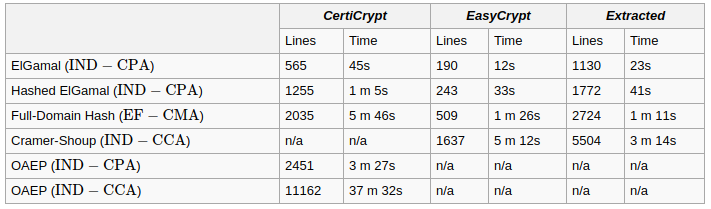
\includegraphics[width=.8\textwidth]{tabla_1}
  \caption{}
  \label{fig:simple}
\end{figure}
\begin{thebibliography}{8}
\bibitem{ref_article1}
Gilles Barthe, Juan Manuel Crespo, Benjamin Gregoire, Cesar Kunz, Santiago Zanella Beguelin. Computer-Aided Cryptographic Proofs. Third International Conference, 2012.
\bibitem{ref_webpage1}
OCaml Website: (2013) https://ocaml.org.
\bibitem{ref_book1}
G. Barthe, B. Grégoire, and S. Zanella Béguelin, “Probabilistic relational hoare
logics for computer-aided security proofs,” in Mathematics of Program Construction
(J. Gibbons and P. Nogueira, eds.), vol. 7342 of Lecture Notes in
Computer Science, pp. 1–6, Springer Berlin Heidelberg, 2012.
\bibitem{ref_webpage2}
Proof-General Website: (2016) https://proofgeneral.github.io.
\bibitem{ref_article3}
Bellare, M., Rogaway, P.: The security of triple encryption and a framework for
code-based game-playing proofs. In: EUROCRYPT 2006. LNCS, vol. 4004, pp.
409–426. Springer (2006)
\bibitem{ref_article4}
Backes, M., Berg, M., Unruh, D.: A formal language for cryptographic pseudocode.
In: LPAR 2008. LNCS, vol. 5330, pp. 353–376. Springer (2008)


%\bibitem{ref_book1}
%Jonathan Katz, Yehuda Lindell: Introduction to modern cryptography. 2nd edn. CHAPMAN \& HALL/CRC, Boca Raton, FL (2008).
\end{thebibliography}
\end{document}
\grid


